% Springer Nature / Cluster Computing planning manuscript
% Version 0.1 -- paragraph-level research and writing plan
% Requires sn-jnl.cls from the official Springer Nature journal template (v3.1, Dec. 2024).
\documentclass[pdflatex,sn-mathphys-num,iicol]{sn-jnl}

\usepackage{graphicx}
\usepackage{multirow}
\usepackage{amsmath,amssymb,amsfonts}
\usepackage{amsthm}
\usepackage{xcolor}
\usepackage{textcomp}
\usepackage{booktabs}
\usepackage{tabularx}
\usepackage{array}
\usepackage{adjustbox}
\usepackage[section]{placeins}
\usepackage{dblfloatfix}
\usepackage{listings}
\usepackage{enumitem}
\usepackage{url}
\setlength{\emergencystretch}{2em}
\Urlmuskip=0mu plus 1mu

\newcolumntype{Y}{>{\raggedright\arraybackslash\hspace{0pt}}X}
\newcolumntype{R}{>{\raggedleft\arraybackslash\hspace{0pt}}X}
\newcolumntype{C}{>{\centering\arraybackslash\hspace{0pt}}X}
\newcommand{\placeholder}[1]{\textcolor{red!75!black}{[TODO:\allowbreak{} #1]}}
\newcommand{\resultplaceholder}[1]{\textcolor{red!75!black}{[RESULT: #1]}}
\newcommand{\citeplaceholder}[1]{\textcolor{purple!80!black}{[CITATION NEEDED: #1]}}
\newcommand{\decisionplaceholder}[1]{\textcolor{orange!80!black}{[DECISION: #1]}}
\newcommand{\newtext}[1]{\textcolor{red}{#1}}
% Drafting notes remain in the source but are suppressed in the rendered paper.
\newcommand{\tpexplain}[1]{}
\newcommand{\figureplaceholder}[2]{%
  \begin{figure}[!htbp]
  \centering
  \fbox{\begin{minipage}[c][3.2cm][c]{0.90\columnwidth}
  \centering\textbf{FIGURE PLACEHOLDER: #1}\par\medskip
  \raggedright #2
  \end{minipage}}
  \caption{#1.}
  \label{fig:#1}
  \end{figure}}
\newcommand{\widefigureplaceholder}[2]{%
  \begin{figure*}[!htbp]
  \centering
  \fbox{\begin{minipage}[c][4.0cm][c]{0.91\textwidth}
  \centering\textbf{FIGURE PLACEHOLDER: #1}\par\medskip
  \raggedright #2
  \end{minipage}}
  \caption{#1.}
  \label{fig:#1}
  \end{figure*}}

\theoremstyle{plain}
\newtheorem{theorem}{Theorem}
\newtheorem{proposition}[theorem]{Proposition}
\newtheorem{corollary}[theorem]{Corollary}
\newtheorem{lemma}[theorem]{Lemma}
\theoremstyle{definition}
\newtheorem{definition}{Definition}
\theoremstyle{remark}
\newtheorem{remark}{Remark}

\raggedbottom
\setlength{\tabcolsep}{3pt}

\begin{document}

\title[Commit-Then-Sample Sparse JL for ZK Clustering]{Commit-Then-Sample Sparse Johnson--Lindenstrauss Transforms for Efficient Zero-Knowledge Clustering}

\author*[1]{\fnm{First} \sur{Author}}\email{\placeholder{email}}
\author[2]{\fnm{First} \sur{Coauthor}}\email{\placeholder{email}}
\affil*[1]{\orgdiv{Department of Computer Engineering}, \orgname{Sharif University of Technology}, \orgaddress{\city{Tehran}, \country{Iran}}}
\affil[2]{\orgdiv{\placeholder{department}}, \orgname{\placeholder{institution}}, \orgaddress{\city{\placeholder{city}}, \country{\placeholder{country}}}}

\abstract{Zero-knowledge proofs can verify clustering over private high-dimensional data, but repeated distance calculations may dominate prover cost. \emph{CommitJL} binds the dataset and public clustering parameters before a verifier challenge selects a sparse finite-field-friendly Johnson--Lindenstrauss transform. This order prevents post-challenge adaptation within an eligible commitment and reduces projection to signed additions; a task-level commitment budget limits grinding across repeated attempts. The proof establishes correct execution in the projected space, while a separate geometric argument relates the result to the original data. We give preservation conditions for fixed-center clustering cost, nearest-centroid assignments, and density neighborhoods. The planned evaluation compares full dimension, principal component analysis, dense and sparse random projections and coordinate sampling on synthetic and real datasets; the cited deterministic ZK-oriented projection remains outside the measured comparison. \resultplaceholder{Replace with the principal quantitative result, fidelity result, and tested backend before submission.}}

\keywords{zero-knowledge proofs, dimensionality reduction, Johnson--Lindenstrauss transform, clustering, ZKML, privacy-preserving computation}

\maketitle

% AUTHORING NOTE: Every blue TEMPLATE EXPLANATION paragraph is drafting
% scaffolding and must be removed before submission. Red RESULT/PLACEHOLDER
% fields require measurements or author decisions. Purple CITATION NEEDED
% fields form a citation checklist. Recount the abstract after inserting results.
% The final manuscript should keep at most three heading levels, cite every
% table and figure in numerical order, and replace boxed figure descriptions
% with original vector or high-resolution artwork.

\section{Introduction}\label{sec:introduction}

\tpexplain{Paragraph 1 --- establish the practical problem. Begin with private high-dimensional clustering as a recurring building block in outsourced analytics, biometric or medical analysis, fraud detection, and collaborative learning. End with the verification need; cite ZK and privacy-preserving analytics surveys.}
Clustering sensitive records creates two requirements that are often in tension: the analyst must keep the records private, and the party relying on the result must be able to check the computation. This setting arises when records contain medical measurements, behavioral profiles, learned embeddings, or proprietary telemetry. Zero-knowledge (ZK) proofs can establish that a specified computation was carried out without revealing its private inputs \cite{gmr1991knowledge,zkmlsurvey2026,zkcnn2021}.

\tpexplain{Paragraph 2 --- quantify the bottleneck. Explain why distances in dimension d are expensive and distinguish native computation from proving cost. Insert a motivating profile from the implemented backend.}
The difficulty is proof cost. For $n$ points, $k$ candidate centroids, and dimension $d$, one assignment step already evaluates $\Theta(nkd)$ coordinate contributions. A ZK circuit must also constrain ranges, compare distances, and materialize witnesses, so fast native linear algebra does not imply a cheap proof \cite{zkcnn2021,ezdps2023}. Whether distance and comparison gadgets dominate in the selected backend is therefore measured rather than assumed.

\tpexplain{Paragraph 3 --- introduce JL but immediately expose the security subtlety. The novelty setup is commit first, sample second.}
A Johnson--Lindenstrauss (JL) transform maps points from $\mathbb{R}^d$ to $\mathbb{R}^m$, with $m\ll d$, while approximately preserving pairwise distances \cite{johnson1984extensions,achlioptas2003database,kane2014sparser}. This suggests reducing the dimension before proving repeated distance computations. The usual JL guarantee, however, fixes the point set before drawing an independent transform. A prover that sees the transform first can instead choose data in its kernel or in a badly distorted subspace. The protocol order must match the order assumed in the geometric argument.

\tpexplain{Paragraph 4 --- one crisp system sentence and one crisp separation of guarantees. Name the system only after checking trademark/name collisions.}
CommitJL first binds the prover to the private dataset and fixes the public clustering parameters; only then does fresh randomness select a sparse signed projection. The ZK proof checks matrix authentication, projection, and the subsequent clustering computation. A separate geometric argument relates the projected answer to the original-space problem. Keeping these claims separate matters: proof soundness concerns correct execution in the projected space, whereas geometric fidelity concerns the quality of the approximation.

\tpexplain{Paragraph 5 --- list contributions as falsifiable claims, not features. Replace every result field after evaluation.}
This paper makes four contributions:
\begin{enumerate}[leftmargin=*]
  \item a commit-then-sample threat model that fixes both private data and public clustering parameters before the projection challenge, with an explicit bound on repeated commitments;
  \item a canonical sparse $\{-1,0,+1\}$ projection format and matrix-authentication path that avoids variable-length sampling inside the circuit;
  \item clustering-specific guarantees, including projected $k$-means cost, a nearest-centroid margin condition, and a DBSCAN neighborhood-margin extension; and
  \item an evaluation over eight fixed native corpora and resource-bounded proof workloads, reporting fidelity, setup/proving trade-offs, and failures without claiming a general sparse-over-full proving speedup.
\end{enumerate}

\tpexplain{Paragraph 6 --- roadmap. Keep this short and aligned exactly with the final section order.}
The remainder of the paper reviews the closest work, defines the protocol and its guarantees, and then evaluates proof cost and clustering fidelity before discussing limitations.

\newtext{\begin{figure*}[!htbp]
\centering
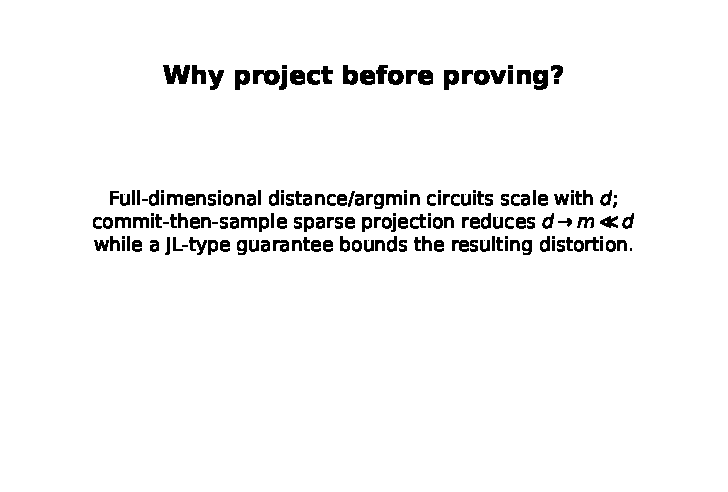
\includegraphics[width=0.91\textwidth]{figures/motivation.pdf}
\caption{Motivation and cost bottleneck.}
\label{fig:Motivation and cost bottleneck}
\end{figure*}}

\subsection{Background, model, and problem statement}\label{sec:background}

\subsubsection{Notation and verifiable clustering}
\tpexplain{Paragraph 1 --- define every symbol used later. Table~\ref{tab:notation} is authoritative; keep symbols consistent across equations, pseudocode, and code.}
Let $X=[\mathbf{x}_1,\ldots,\mathbf{x}_n]^\top\in\mathbb{Z}^{n\times d}$ denote the private, quantized dataset, $A\in\{-1,0,+1\}^{m\times d}$ the public unnormalized sparse transform, $P=A/\sqrt q$ the corresponding real embedding, and $Z=XA^\top\in\mathbb{Z}^{n\times m}$ the circuit representation. The field used by the proof system is $\mathbb{F}_p$. Signed integers are represented canonically within a bounded interval embedded in $\mathbb{F}_p$.

\begin{table}[!htbp]
\caption{Notation and ownership of protocol values.}\label{tab:notation}
\centering\scriptsize
\begin{tabularx}{\columnwidth}{@{}Y Y Y@{}}
\toprule
Symbol/domain & Meaning & Visibility \\
\midrule
$n,d,m,k\in\mathbb N$ & points, input/projected dimensions, clusters & public \\
$X\in\mathbb Z^{n\times d}$ & quantized dataset & private \\
$C_X,C_\theta,C_A$ & data commitment and parameter/matrix digests & public \\
$s,\rho\in\{0,1\}^{\lambda}$ & projection seed and fresh challenge & public \\
$A,P=A/\sqrt q$ & circuit matrix and real embedding & witness/derived \\
$q,Q\in\mathbb N$ & column sparsity and task attempt budget & public \\
$Z\in\mathbb Z^{n\times m}$ & projected points & private \\
$\mathcal C,a_i$ & fixed centers and assignment & public/private \\
$\epsilon,\delta\in(0,1)$ & distortion and failure targets & public \\
$p,B$ & field modulus and coordinate bound & public \\
\bottomrule
\end{tabularx}
\end{table}

\subsubsection{Proof statement and privacy boundary}
\tpexplain{Paragraph 1 --- state the exact NP relation. Avoid saying “prove clustering” without specifying public input, witness, algorithm steps, iteration count, and tie-breaking.}
The primary statement is a fixed-centroid assignment-and-cost audit. Before the challenge, the prover publishes $C_X$ and the verifier records the public parameter digest $C_\theta=H_\theta(\mathsf{Encode}(\mathcal C,m,q,\mu))$, where $\mathcal{C}=\{c_1,\ldots,c_k\}\subset\mathbb Z^d$. After receiving fresh $\rho$, the verifier derives $s=H(\texttt{CommitJL-v1}\|C_X\|C_\theta\|\rho)$, expands the canonical sparse matrix $A$, and computes $C_A=H_A(\mathsf{Encode}(A))$. The public input is $(C_X,C_\theta,C_A,\mu,\rho,m,q,\mathcal C,\widehat\Psi)$; the witness contains $(X,r_X,A,a_1,\ldots,a_n)$ and authentication data. The circuit accepts only if (i) $C_X$ opens to the canonical encoding of $X$ and its dimensions and scale; (ii) $H_\theta(\mathsf{Encode}(\mathcal C,m,q,\mu))=C_\theta$ and the canonical supplied sparse list hashes to $C_A$; (iii) every coordinate and accumulator satisfies the signed range; (iv) each $a_i$ is the lowest-index minimizer of $\|A(x_i-c_j)\|_2^2$; and (v) $\widehat\Psi=\sum_i\|A(x_i-c_{a_i})\|_2^2$. The normalized projected cost is $\widehat\Psi/q$ in the external analysis; no field division or divisibility assumption is used. Assignments and projected values remain private.

\begin{table*}[!htbp]
\caption{Statement variants and their privacy--cost trade-offs.}\label{tab:statements}
\centering\small
\begin{adjustbox}{max width=\textwidth}
\begin{tabularx}{\textwidth}{@{}Y Y Y Y@{}}
\toprule
Variant & Public output & Private witness & Main implication \\
\midrule
Nearest public centroids & assignments or class IDs & $X$, projected points, distances & simplest circuit; centroids may reveal model \\
Private centroids & assignments and centroid commitment & $X$, centroids, distances & stronger privacy; requires proving centroid consistency \\
Fixed-iteration $k$-means & final centroid commitment and optional assignments & $X$, all $T$ iterations & realistic but comparison- and division-heavy \\
Audited clustering cost & claimed objective and commitment to assignments & $X$, assignments, centroids & proves cost for an externally supplied clustering \\
DBSCAN extension & labels/core-point flags or their commitment & $X$, neighborhood bits, traversal witness & quadratic pairs unless neighbor search is constrained \\
\bottomrule
\end{tabularx}
\end{adjustbox}
\end{table*}

\subsubsection{Threat model and commit-then-sample requirement}
\tpexplain{Paragraph 1 --- enumerate malicious capabilities and explicit non-goals. Say who supplies randomness and what must be unpredictable at commitment time.}
We consider a malicious prover that may choose arbitrary private data, witnesses, and messages, but cannot break commitment binding, collision resistance, the XOF assumption, or proof-system knowledge soundness. The verifier follows the challenge and verification rules but may try to infer information from public outputs. Both $C_X$ and $C_\theta$ must be fixed before the projection seed receives entropy unavailable to the prover. Commit-and-prove systems such as Artemis motivate binding externally committed values to a proved computation \cite{artemis2024}. A task admits at most $Q$ eligible commitments from an authenticated prover; eligibility is fixed by a public log or deadline before the challenge source is known. The single-attempt model has $Q=1$, and all task-level failure bounds state their dependence on $Q$. Output privacy, maliciously selected centroids outside the recorded parameter digest, unbounded recommitment, denial of service, and differential privacy remain outside the claimed guarantees.

\begin{table*}[!htbp]
\caption{Threats, assumptions, and protocol responses.}\label{tab:threats}
\centering\small
\begin{adjustbox}{max width=\textwidth}
\begin{tabularx}{\textwidth}{@{}Y Y Y@{}}
\toprule
Threat or failure & Required assumption/check & Response in design/evaluation \\
\midrule
Input or centers chosen after seeing $A$ & binding data commitment; recorded parameter digest; fresh challenge & enforce $(C_X,C_\theta)\rightarrow\rho\rightarrow A$ order \\
Prover substitutes another dataset & commitment opening verified in circuit or via authenticated access & bind dimensions, scale, ordering, and values into $C_X$ \\
Grinding across commitments & identifiable entropy; public eligibility rule; budget $Q$ & report $Q$ and scale the task-level bound by $Q$ \\
Finite-field wraparound & sound range bounds for inputs, projections, and squared distances & prove bounds; select $p$ with safety margin \\
Matrix substitution & collision-resistant $H_A$; canonical sparse-list encoding & verifier derives $A$; circuit authenticates its digest \\
Projection reveals private information & leakage depends on whether $Z$ is public & keep $Z$ private in primary protocol; report disclosure variant separately \\
Approximation changes clustering & geometric assumptions are separate from proof soundness & report fidelity and certified-margin coverage \\
\bottomrule
\end{tabularx}
\end{adjustbox}
\end{table*}

\newtext{\begin{figure*}[!htbp]
\centering
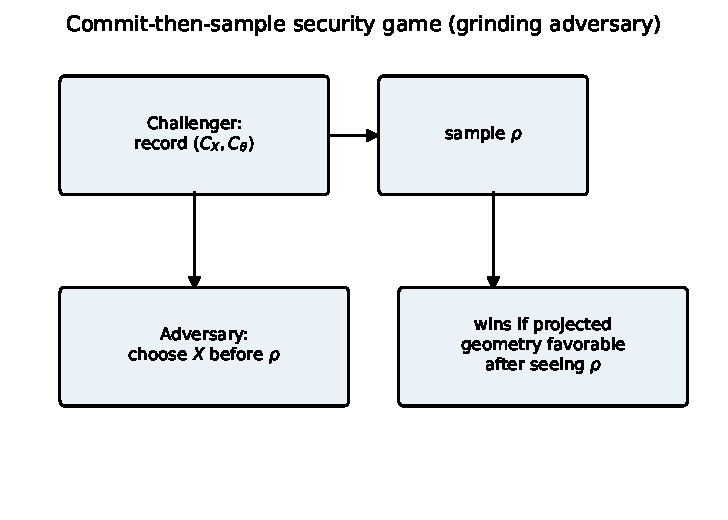
\includegraphics[width=0.91\textwidth]{figures/security_game.pdf}
\caption{Security game for adaptive projection attacks.}
\label{fig:Security game for adaptive projection attacks}
\end{figure*}}

\subsubsection{Clustering objectives}
\tpexplain{Paragraph 1 --- define the primary algorithm. Prefer nearest-centroid or assignment/cost verification for the first prototype; full Lloyd iteration is an explicit scope decision.}
For centroids $\mathcal{C}=\{\mathbf{c}_1,\ldots,\mathbf{c}_k\}$, nearest-centroid assignment is
\begin{equation}
a_i=\arg\min_{j\in[k]}\|\mathbf{x}_i-\mathbf{c}_j\|_2^2,
\end{equation}
with deterministic lowest-index tie-breaking. The $k$-means objective is
\begin{equation}
\Phi_X(\mathcal{C})=\sum_{i=1}^{n}\min_{j\in[k]}\|\mathbf{x}_i-\mathbf{c}_j\|_2^2.
\end{equation}
The primary implementation proves the fixed-centroid assignments and their aggregate projected cost. This scope avoids conflating dimensionality reduction with the separate difficulty of proving centroid division and convergence; fixed-iteration Lloyd training and DBSCAN are modular extensions.

\section{Related work}\label{sec:related}

\tpexplain{Opening paragraph --- explain the organizing dimensions. Table~\ref{tab:related-a} should make the novelty gap inspectable rather than relying on adjectives.}
Four lines of work delimit the problem: ZK machine-learning systems determine what is practical to prove; JL and clustering sketches provide approximation guarantees; cryptographic uses of projection clarify what projection alone does not prove; and deterministic proof-oriented projections offer the closest systems baseline. Table~\ref{tab:related-a} compares these lines by protocol order, transform cost, clustering guarantee, and end-to-end evaluation.

\begin{table*}[!htbp]
\caption{Comparison with the closest lines of work.}\label{tab:related-a}
\centering\scriptsize
\begin{adjustbox}{max width=\textwidth}
\begin{tabularx}{\textwidth}{@{}Y Y Y Y Y@{}}
\toprule
Work/family & Projection & ZK computation & Clustering-specific guarantee & Gap addressed here \\
\midrule
JL lemma and sparse JL \cite{johnson1984extensions,achlioptas2003database,kane2014sparser} & random dense/sparse & no & distance preservation & circuit cost and adversarial ordering absent \\
Clustering sketches \cite{cohen2015dimensionality,makarychev2019performance} & random embedding & no & $k$-means/$k$-median cost & no cryptographic realization \\
ezDPS \cite{ezdps2023} & data-dependent PCA & yes & pipeline-dependent & PCA proof cost and adaptive-JL issue differ \\
Commit-and-prove ZKML \cite{artemis2024} & no clustering projection & yes & application-dependent & binds external data/models, but does not study JL fidelity \\
Pisot-$\beta$ ZK projection \cite{dey2026pisot} & deterministic/public reproducible & yes & conditional squared-norm estimator bound & different randomness and adversarial model \\
This work & post-commit sparse signed JL & yes & cost plus assignment/neighborhood margins & combines security order, geometry, and proof cost \\
\bottomrule
\end{tabularx}
\end{adjustbox}
\end{table*}

\subsection{ZK machine learning and private analytics}
\tpexplain{Two paragraphs. First map generic ZKML compilers and specialized systems; second focus on PCA/clustering. Cite performance claims only after checking artifact versions and hardware.}
General-purpose ZK compilers and specialized ZKML systems reduce inference-proof cost through quantization, lookup arguments, polynomial commitments, and operator-specific protocols \cite{zkmlsurvey2026,zkcnn2021,artemis2024}. Their results also show why operation counts alone are insufficient: arithmetic representation and the selected backend determine the cost of an operator.

ezDPS provides a ZK pipeline for principal-component analysis and classification and is therefore the relevant data-dependent dimensionality-reduction baseline \cite{ezdps2023}. CommitJL asks a narrower question: can a data-oblivious sparse embedding selected after commitment reduce clustering-proof cost without unacceptable geometric error? Accordingly, the comparison is limited to systems that expose a reproducible dimensionality-reduction or proof-cost baseline; it is not intended as a survey of privacy-preserving $k$-means.

\subsection{Dimensionality reduction for clustering}
\tpexplain{One paragraph on classical JL, one on clustering-specific projection dimensions. State theorem parameters accurately and separate pairwise preservation from objective preservation.}
Classical JL embeddings preserve all pairwise distances in a fixed set with target dimension logarithmic in the set size and quadratic in the inverse distortion \cite{johnson1984extensions}. Sparse constructions reduce application time while retaining similar embedding guarantees \cite{kane2014sparser}. Clustering-specific analyses can require dimension depending on $k$ and $\epsilon$ rather than directly on $n$ \cite{cohen2015dimensionality,makarychev2019performance}. Our design uses these results as mathematical interfaces, but does not apply their bounds until the implemented distribution satisfies the cited hypotheses.

\subsection{Random projection inside cryptographic protocols}
\tpexplain{Clarify that projection is not itself novel in cryptography. Contrast its role in norm compression with proof-cost-aware ML compression.}
Projection has appeared in cryptographic norm-compression settings, but those objectives and soundness arguments do not establish fidelity of a downstream clustering computation. The closest directly comparable ZK-oriented proposal derives a deterministic projection from a Pisot-$\beta$ orbit and gives a conditional norm-estimation analysis; because it uses public reproducible structure instead of post-commit randomness, it is a relevant literature comparator with a different adversarial model; a verified reproduction was unavailable in the present empirical study \cite{dey2026pisot}.

\section{Methodology}\label{sec:design}

\subsection{CommitJL design and protocol overview}
\tpexplain{Walk through Figure~\ref{fig:Protocol overview} in message order. Specify which computations occur inside versus outside the circuit.}
The protocol has six stages: binding the data and public parameters; sampling the challenge; deterministic sparse-matrix expansion by the verifier; authentication of the sparse matrix inside the circuit; checked projection and clustering; and proof generation. The primary construction authenticates a verifier-derived sparse list through $C_A$. This keeps variable-length rejection sampling outside the fixed circuit while still preventing the prover from substituting another matrix. In-circuit regeneration is an optional variant and requires a separate bounded, circuit-compatible generator.

\newtext{\begin{figure*}[!htbp]
\centering
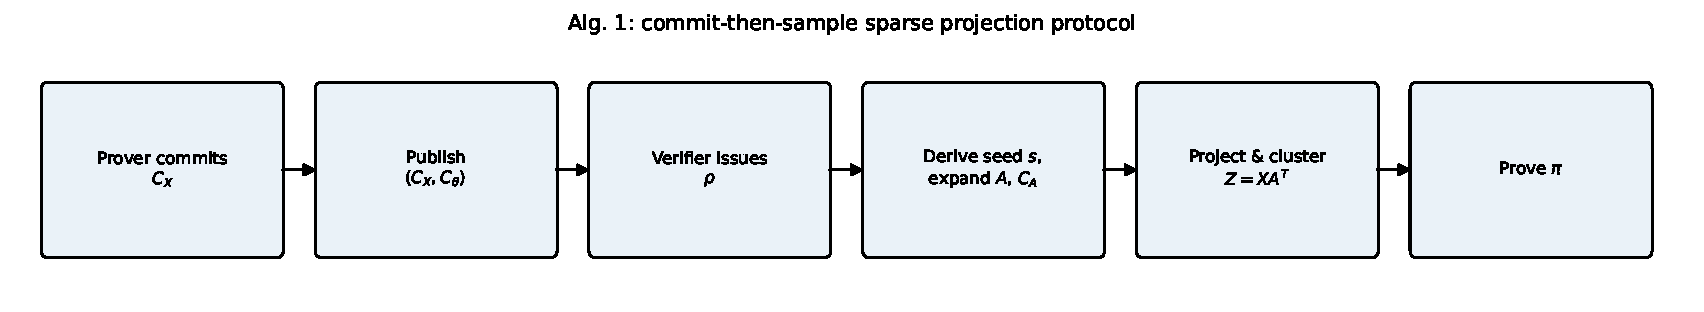
\includegraphics[width=0.91\textwidth]{figures/protocol.pdf}
\caption{Protocol overview.}
\label{fig:Protocol overview}
\end{figure*}}

\begin{figure}[!htbp]
\centering
\begin{minipage}{0.95\columnwidth}\small
\textbf{Algorithm 1: Commit-then-sample sparse projection protocol}\label{alg:commitjl}
\begin{enumerate}[leftmargin=*,nosep]
\item \textbf{Input:} private integer data $X$; public metadata $\mu$; public clustering parameters $\theta=(\mathcal C,m,q)$.
\item $(C_X,r_X)\gets\mathsf{Commit}(\mathsf{Encode}(X,\mu))$.
\item Publish $(C_X,C_\theta)$, where $C_\theta=H_\theta(\mathsf{Encode}(\theta,\mu))$, before learning $\rho$.
\item $s\gets H(\texttt{CommitJL-v1}\|C_X\|C_\theta\|\rho)$.
\item The verifier derives $A\gets\mathsf{SparseMatrixGen}(s,m,d,q)$ and $C_A\gets H_A(\mathsf{Encode}(A))$; $P=A/\sqrt q$ is used only in the real-valued analysis.
\item $Z\gets XA^\top$ using signed integer semantics.
\item $y\gets\mathsf{Cluster}(Z,\theta)$.
\item $\pi\gets\mathsf{Prove}(C_X,C_\theta,C_A,\rho,\theta,y;X,r_X,A,Z,\omega)$.
\item \textbf{Return:} $(C_X,C_\theta,C_A,\rho,\theta,y,\pi)$.
\end{enumerate}
\end{minipage}
\caption{Pseudocode for the proposed protocol.}
\end{figure}

\subsection{Sparse matrix generation}
\tpexplain{Define one exact distribution rather than saying “sparse JL.” State normalization and how it is represented without irrational constants.}
Assume $1\le q\le m$. For each input coordinate $t\in[d]$, domain-separated XOF expansion of $s$ samples an ordered $q$-tuple of \emph{distinct} rows by rejection sampling without replacement, followed by independent sign bits $\sigma_\ell(t)\in\{-1,+1\}$. Rejection removes duplicate rows within a column and modulo bias: a candidate word $u$ is accepted only if $u<2^b-(2^b\bmod m)$, after which the row is $u\bmod m$. Every column of $A$ therefore has exactly $q$ signed unit entries. Because the number of XOF words consumed is variable, the primary circuit does not reproduce this loop. The verifier expands the complete canonical sparse list, while the circuit hashes the supplied list and checks $C_A$ before using any entry. The unnormalized projection is
\begin{equation}
z_r=\sum_{t=1}^{d}\sum_{\ell=1}^{q}\mathbf{1}[h_\ell(t)=r]\,\sigma_\ell(t)x_t.
\end{equation}
The mathematical embedding is $P=A/\sqrt q$, but the circuit never represents the irrational normalization. It compares unnormalized squared distances, whose common factor cancels, and reports the integer cost $\widehat\Psi$; analysis divides by $q$. The byte encoding fixes the XOF, domain tags, word width, rejection rule, column order, sign-bit order, and sparse-list serialization. Sparse-JL literature motivates the construction \cite{kane2014sparser}, but no distribution-specific target-dimension bound is imported without proof: the theorem below is conditional on an explicitly defined embedding event for this generator.

\begin{proposition}[Unbiased squared norm]\label{prop:unbiased-a}
For any fixed $v\in\mathbb R^d$, if the sign bits are mutually independent and uniform in $\{-1,+1\}$ and independent of the sampled rows, then
\[
\mathbb E_A\!\left[q^{-1}\|Av\|_2^2\right]=\|v\|_2^2.
\]
\end{proposition}
The proof is in Appendix~\ref{app:geometry-a}. Unbiasedness alone is not a JL tail bound; the required simultaneous concentration event remains explicit in Theorem~\ref{thm:composition-a}.

\begin{table*}[!htbp]
\caption{Projection baselines and circuit-relevant characteristics.}\label{tab:transforms}
\centering\small
\begin{adjustbox}{max width=\textwidth}
\begin{tabularx}{\textwidth}{@{}Y Y Y Y Y@{}}
\toprule
Transform & Coefficients & Expected nonzeros & In-circuit operations & Security/order note \\
\midrule
No reduction & identity & $d$ per point & downstream cost only & exact baseline \\
Gaussian JL & real/quantized & $md$ & multiply--accumulate & sampled after commitment \\
Rademacher JL & $\{-1,+1\}$ & $md$ & signed additions & sampled after commitment \\
Achlioptas & $\{-1,0,+1\}$ & distribution-dependent & sparse signed additions & sampled after commitment \\
Sparse JL & hashed signs/buckets & $qd$ & $qd$ additions & primary candidate \\
Coordinate sampling & $\{0,1\}$ & $m$ & copies/selects & cheap naive baseline \\
PCA & quantized dense & $md$ & multiply--accumulate plus PCA proof if learned & data-dependent baseline \\
\bottomrule
\end{tabularx}
\end{adjustbox}
\end{table*}

\newtext{\begin{figure}[!htbp]
\centering
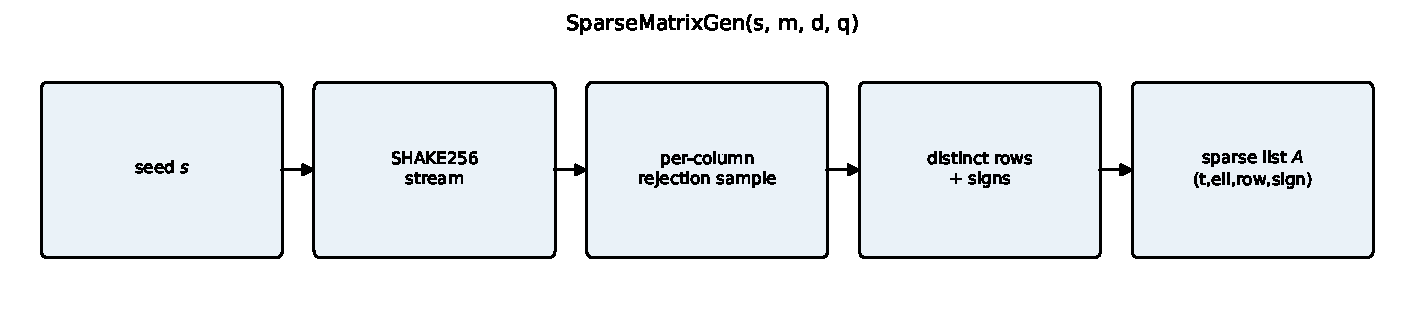
\includegraphics[width=0.90\columnwidth]{figures/generator.pdf}
\caption{Sparse projection generator.}
\label{fig:Sparse projection generator}
\end{figure}}

\subsection{Circuit realization and checked arithmetic}
\tpexplain{Describe exact gadgets and state which operations are constraints versus witness-generation work. Include range checks even if they are costly.}
Signed coefficients eliminate general scalar multiplications: each nonzero contributes either $+x_t$ or $-x_t$ to an accumulator. The circuit verifies the data commitment and $C_A$, checks that the sparse list has exactly one ordered record for each $(t,\ell)$ with valid distinct rows within a column and signs in $\{-1,+1\}$, constrains each accumulator, and range-checks projected differences before squaring. For nearest-centroid assignment, it evaluates $m$ coordinate differences per point--centroid pair, accumulates squared distances, and applies a deterministic less-than gadget.

\begin{table*}[!htbp]
\caption{Symbolic circuit model only; measured total constraints are reported separately. Per-gadget measured attribution is unavailable.}\label{tab:circuit-cost}
\centering\small
\begin{adjustbox}{max width=\textwidth}
\begin{tabularx}{\textwidth}{@{}Y Y Y Y Y@{}}
\toprule
Component & Invocation count & Arithmetic constraints & Lookup/range constraints & Notes \\
\midrule
Commitment authentication & $nd$ leaves, padded to $N$ & $NC_{\rm leaf}+(N-1)C_{\rm node}$ & leaf bounds & leaf and internal-node hashes both counted \\
Matrix authentication & $qd$ sparse records & hash-dependent & row/sign/distinctness checks & verifier performs XOF rejection outside circuit \\
Sparse projection & implemented routing scans $(n+k)mdq$ slots & backend-dependent selector/addition cost & accumulator bounds & $nqd$ is an algorithmic ideal, not measured circuit cost \\
Projected squared distance & $nkm$ coordinates & $nkm$ squarings and $nk(m-1)$ additions & $nkm$ difference bounds & public centroids projected once \\
Argmin & $n(k-1)$ comparisons & backend-specific & bit decomposition/lookups & tournament with lowest-index ties \\
Centroid update & not implemented & not measured & not measured & outside fixed-center proof scope \\
Full-dimensional baseline & $nkd$ coordinates & $nkd$ squarings and $nk(d-1)$ additions & $nkd$ difference bounds & reference point \\
\bottomrule
\end{tabularx}
\end{adjustbox}
\end{table*}

\newtext{\begin{figure*}[!htbp]
\centering
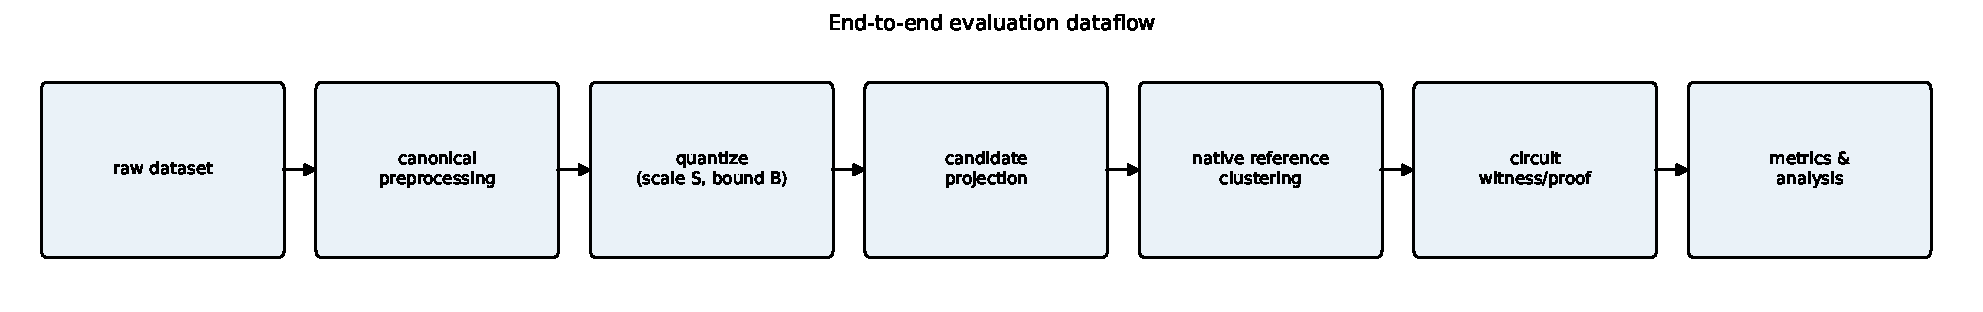
\includegraphics[width=0.91\textwidth]{figures/dataflow.pdf}
\caption{Circuit dataflow and constraint hotspots.}
\label{fig:Circuit dataflow and constraint hotspots}
\end{figure*}}

\subsection{Randomness instantiations}
\tpexplain{Give deployable alternatives and state the trust/freshness assumption for each. Select one primary instantiation for experiments.}
We consider three challenge sources: a verifier nonce, a public randomness beacon referenced by round, and a two-party commit--reveal coin flip. Deriving the seed from $C_X$ alone is deterministic and permits offline search over commitment randomness. The primary protocol therefore uses a fresh 256-bit verifier nonce after $(C_X,C_\theta)$ has entered the task log. A nonce is single-use, and the log admits at most $Q$ eligible commitments per authenticated prover and task. A new commitment consumes another attempt; it does not reset the analysis. A beacon with a commitment deadline gives the cleanest public enforcement, while commit--reveal avoids trusting either party as the sole entropy source.

\subsection{Geometric and cryptographic guarantees}\label{sec:theory}

\subsubsection{Separation of soundness and fidelity}
\tpexplain{State a composition theorem with explicit assumptions. Do not imply that ZK soundness proves the JL event.}
Define $D(X,\mathcal C)=\{x_i-c_j:i\in[n],j\in[k]\}$ and
let $\mathcal E_\epsilon(A;D)$ be the event that, for every $v\in D$,
\begin{equation*}
(1-\epsilon)\|v\|_2^2
\le q^{-1}\|Av\|_2^2
\le(1+\epsilon)\|v\|_2^2.
\end{equation*}
\begin{theorem}[Soundness--fidelity composition]\label{thm:composition-a}
Suppose (i) the data commitment is computationally binding; (ii) $(C_X,C_\theta)$ becomes ineligible for replacement before fresh $\rho$ is sampled; (iii) $H_\theta$ and $H_A$ are collision resistant; (iv) the proof system is knowledge-sound for the relation in Section~\ref{sec:background}; (v) the verifier and circuit use the same canonical encodings and checked signed-integer semantics; and (vi) $\mathcal E_\epsilon(A;D(X,\mathcal C))$ holds. Then, except with probability at most $\delta_{\rm bind}+\delta_{\rm hash}+\delta_{\rm ks}$, an accepted $\widehat\Psi$ equals the specified unnormalized nearest-centroid cost on the committed $X$ under the verifier-derived $A$. Here $\delta_{\rm hash}$ covers collisions in either digest. Moreover,
\[
(1-\epsilon)\Phi_X(\mathcal C)\le \widehat\Psi/q\le(1+\epsilon)\Phi_X(\mathcal C).
\]
For one eligible commitment and an ideal generator, failure of premise (vi) contributes $\delta_{\rm geom}=\Pr[\neg\mathcal E_\epsilon]$. If this bound holds uniformly for every admissible registered dataset/parameter pair, then across at most $Q$ eligible commitments the union bound gives task-level failure at most $Q(\delta_{\rm bind}+\delta_{\rm hash}+\delta_{\rm ks}+\delta_{\rm geom}+\operatorname{Adv}_{\rm xof})$. No numerical value is asserted until the primitives, generator model, admissible input class, and task policy are instantiated.
\end{theorem}
The proof is given in Appendix~\ref{app:security-a}; the cost inequality is proved in Appendix~\ref{app:geometry-a}. Cryptographic acceptance and geometric approximation are separate claims.

\subsubsection{Clustering-cost preservation}
\tpexplain{Use the strongest applicable theorem from the clustering-sketch literature, with exact constants/conditions copied and cited after verification.}
For the primary fixed public center set $\mathcal C$, let $S=X\cup\mathcal C$. If the realized transform preserves every squared distance in $S$ within $1\pm\epsilon$, then summing the point-to-assigned-center inequalities gives
\begin{equation}
(1-\epsilon)\Phi_X(\mathcal C)\le q^{-1}\Phi_{AX}(A\mathcal C)\le(1+\epsilon)\Phi_X(\mathcal C).
\end{equation}
This statement requires no claim about recovering an optimal center set. Stronger results that preserve an optimum or all candidate clusterings require the precise projection-cost-preserving sketch hypotheses in the cited clustering literature \cite{cohen2015dimensionality,makarychev2019performance}; they are evaluated separately and are not used to justify the primary audit.

\subsubsection{Nearest-centroid margin}
\tpexplain{This is a simple but useful exact-decision theorem. Define the closest and runner-up distances and handle zero distance/ties.}
Let $d_1<d_2$ be the original distances from a query point to its closest and second-closest centroids. Under squared-distance distortion $1\pm\epsilon$, the assignment is unchanged whenever
\begin{equation}
\frac{d_2^2}{d_1^2}>\frac{1+\epsilon}{1-\epsilon}.
\label{eq:centroid-margin}
\end{equation}
This condition yields a per-point certificate: points satisfying Eq.~\eqref{eq:centroid-margin} are guaranteed stable under the embedding event, while other points are empirically evaluated rather than declared incorrect.

\figureplaceholder{Nearest-centroid margin geometry}{A 2D explanatory schematic with query $x$, closest centroid $c_1$, runner-up $c_2$, original radii $d_1,d_2$, and projected distortion envelopes. Include Eq. (nearest-centroid margin) beside the drawing and a small panel showing certified versus uncertified points as $\epsilon$ changes.}

\subsubsection{DBSCAN neighborhood-margin extension}
\tpexplain{Make DBSCAN an extension unless a scalable neighborhood circuit is implemented. Prove graph preservation first, then inherit deterministic DBSCAN output under fixed ordering/tie rules.}
DBSCAN connects $i$ and $j$ when $\|\mathbf{x}_i-\mathbf{x}_j\|_2\leq\rho$. Under the JL event, pairs with
\begin{equation}
\|\mathbf{x}_i-\mathbf{x}_j\|_2^2\leq\frac{\rho^2}{1+\epsilon}
\end{equation}
remain neighbors, while pairs with
\begin{equation}
\|\mathbf{x}_i-\mathbf{x}_j\|_2^2>\frac{\rho^2}{1-\epsilon}
\end{equation}
remain non-neighbors. Only pairs in the ambiguity band
\begin{equation}
\mathcal{A}_{\epsilon}(\rho)=\left[\frac{\rho^2}{1+\epsilon},\frac{\rho^2}{1-\epsilon}\right]
\end{equation}
may change adjacency.

\begin{corollary}[DBSCAN graph stability]
If no pairwise squared distance lies in $\mathcal{A}_{\epsilon}(\rho)$ and the embedding event holds, the $\rho$-neighborhood graph is identical before and after projection. Therefore deterministic DBSCAN with fixed $\mathrm{minPts}$ and tie/order rules returns the same clustering.
\end{corollary}

\widefigureplaceholder{DBSCAN ambiguity band}{Plot original squared distance on the horizontal axis. Shade guaranteed-neighbor, ambiguous, and guaranteed-nonneighbor intervals around $\rho^2$. Add a second panel with an example neighborhood graph before and after projection, highlighting that exact graph preservation implies exact DBSCAN output.}

\subsubsection{Quantization and no-wraparound conditions}
\tpexplain{Bridge real-valued theorems and field arithmetic. Bound errors from quantization separately from random-projection distortion.}
Let real input coordinates be scaled by $S$ and rounded to integers with per-coordinate error at most $1/(2S)$. Hence $\|x-\widetilde x/S\|_2\le\sqrt d/(2S)$; for a pair $u,v$, the distance perturbation is at most $\sqrt d/S$, and the squared-distance error is at most $2\|u-v\|_2\sqrt d/S+d/S^2$. If $|x_t|,|c_t|\le B$, distinct rows within each column imply that a fixed output row receives at most one contribution per input coordinate. Thus a projected point--centroid coordinate has magnitude at most $2dB$, independent of $q$. Put $D_{\max}=4md^2B^2$ and $\Psi_{\max}=nD_{\max}$. Comparison differences may reach $2D_{\max}$. The implementation range-checks signed values against $M=\max\{2dB,2D_{\max},\Psi_{\max}\}$ and requires $p>2M$; tighter data-dependent bounds may improve performance but cannot replace a proved worst-case certificate.

\begin{table*}[!htbp]
\caption{Theoretical claims, assumptions, and empirical checks.}\label{tab:claims}
\centering\small
\begin{adjustbox}{max width=\textwidth}
\begin{tabularx}{\textwidth}{@{}Y Y Y Y@{}}
\toprule
Claim & Required assumptions & What is formally proved & What is measured \\
\midrule
Projected computation soundness & binding commitment; ZK knowledge soundness; canonical generator & accepted proof corresponds to committed $X$ and derived $A$ & negative tests and transcript conformance \\
Pairwise distance preservation & fixed point set; valid JL distribution; sufficient $m$ & $1\pm\epsilon$ distance event & max/mean/quantile distortion \\
$k$-means cost preservation & exact cited sketch theorem conditions & objective relation specified by theorem & objective ratio and ARI \\
Nearest-centroid stability & pairwise event and Eq.~\eqref{eq:centroid-margin} & unchanged assignment for certified points & certificate coverage and violations \\
DBSCAN stability & no distance in ambiguity band; deterministic implementation & identical neighborhood graph/output & ambiguous-pair rate and ARI \\
Integer equivalence & range checks; quantization error bound & no wraparound; bounded real/integer discrepancy & overflow tests and precision sensitivity \\
\bottomrule
\end{tabularx}
\end{adjustbox}
\end{table*}

\subsection{Implementation}\label{sec:implementation}

\tpexplain{Paragraph 1 --- name versions, curves/fields, commitment hash, proof backend, language, and hardware-neutral design choices. Do not postpone key reproducibility facts to a repository.}
We implement CommitJL in \newtext{gnark v0.16.3 (gnark-crypto v0.21.0), supporting both Groth16 and PLONK backends}, using the \newtext{BN254 scalar field and curve}, \newtext{a MiMC-BN254 (Miyaguchi--Preneel) Merkle-tree/sponge commitment hash}, and \newtext{gnark's \texttt{std/rangecheck} batched-lookup gadget (with a manual bit-decomposition fallback) and \texttt{std/math/cmp} for comparisons}. The host implementation is written in \newtext{Go (go1.27.1) for the circuit and prover/verifier CLI, with the surrounding protocol logic in Python}, while experiment orchestration and clustering metrics use \newtext{Python 3.12.3 with NumPy 2.5.3, SciPy 1.18.1, scikit-learn 1.9.1, and pandas 3.0.6 (exact versions captured per run by \texttt{env\_capture.py} into \texttt{results/headline.json})}. All arithmetic parameters and transcript encodings are fixed in a versioned manifest.

\newtext{The PLONK backend is instantiated with an unsafe, test-only KZG SRS (gnark's \texttt{test/unsafekzg}) suitable only for benchmarking circuit cost, not for a trusted deployment. Of the circuit variants enumerated in \texttt{zk/circuit/circuit.go} (full, sparse, dense, coord, pca-public, pisot, prepublished, incircuit-gen), the sparse, full, prepublished, pca-public, and pisot variants are implemented and exercised by the test suite; the dense and coord variants are implemented but untested; and the incircuit-gen variant, which would rebuild the sparse generator and MiMC XOF inside the circuit, is not yet implemented (it is a stub). In-circuit, the public commitments $C_\theta$ and $C_A$ are checked against a field-native MiMC digest of the centroids/sparse list (\texttt{zk\_bridge.py}'s \texttt{field\_hash\_theta}/\texttt{field\_hash\_sparse\_list}), which differs from \texttt{commit.py}'s host-side byte-packed encoding of the same values; the two are intentionally not required to match.}

\tpexplain{Paragraph 2 --- describe optimizations and make every one independently disableable for ablation.}
The implementation batches signed accumulation, reuses projected centroids where allowed, applies an argmin tournament, and separates matrix generation from projection constraints. Compile-time and run-time switches independently disable sparsity, post-commitment generation, range-check batching, and shared subexpressions, enabling the ablation in Table~\ref{tab:ablation-a}.

\newtext{\begin{figure}[!htbp]
\centering
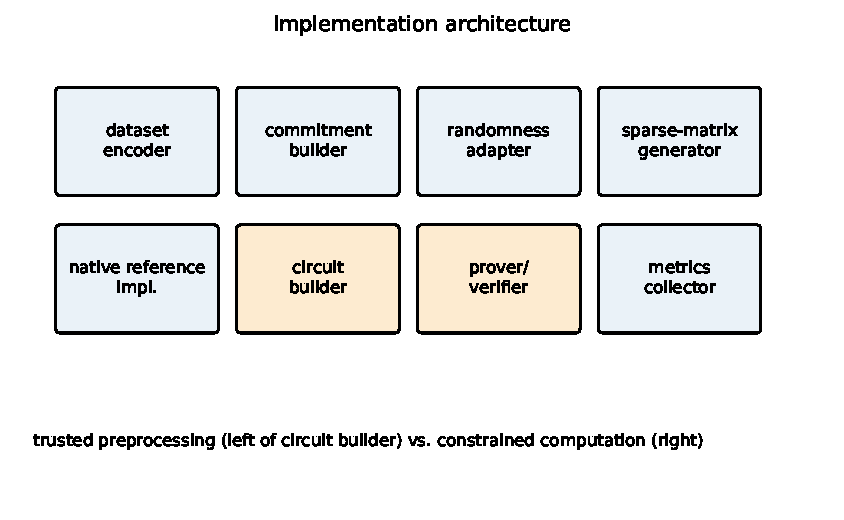
\includegraphics[width=0.90\columnwidth]{figures/architecture.pdf}
\caption{Implementation architecture.}
\label{fig:Implementation architecture}
\end{figure}}

\section{Experimental analysis}\label{sec:method}

\subsection{Research questions}
\tpexplain{Use numbered RQs so every result subsection has one purpose and a declared primary metric.}
\begin{description}[leftmargin=1.3cm,style=nextline]
\item[RQ1] How do projection dimension and sparsity affect geometric and clustering fidelity?
\item[RQ2] How much do candidate projections reduce constraints, proving time, and peak memory?
\item[RQ3] Does commit-then-sample add material overhead relative to a pre-published transform?
\item[RQ4] Do the margin conditions predict assignment and DBSCAN stability?
\item[RQ5] How robust are conclusions to dataset size, original dimension, cluster count, separation, quantization, backend, and hardware?
\end{description}

\subsection{Datasets and controlled generators}
\begin{table*}[!htbp]
\caption{Datasets and their role in the evaluation.}\label{tab:datasets-a}
\centering\scriptsize
\begin{adjustbox}{max width=\textwidth}
\begin{tabularx}{\textwidth}{@{}Y R R R Y Y@{}}
\toprule
Dataset/family & $n$ & $d$ & classes/$k$ & Preprocessing & Why included \\
\midrule
Gaussian mixtures & $2{,}000$ (primary fidelity) & 256, 512 & 5, 8 (latent) & controlled separation, variance, imbalance & known latent labels and tunable margin \\
DBSCAN margin generator & \newtext{300--1{,}000 (config-dependent)} & \newtext{64--128 (config-dependent)} & variable & construct pair distances around $\rho$ & direct test of ambiguity-band theorem \\
MNIST (analyzed subset) & 5,000 & 784 & 10 & scale pixels; fixed split/subsample & standard dense benchmark \\
Fashion-MNIST (analyzed subset) & 5,000 & 784 & 10 & same protocol as MNIST & harder same-shape benchmark \\
Gisette (training subset) & 3,000 & 5,000 & 2 & fixed training split/subset & high-dimensional dense features \\
Arcene (training split) & 100 & 10,000 & 2 & missing-value/scale policy & very high dimension, low sample count \\
20 Newsgroups & \newtext{3,000 (training subset)} & \newtext{2,000 (TF--IDF \texttt{max\_features})} & 20 & TF--IDF; sparse input & sparse high-dimensional text \\
\bottomrule
\end{tabularx}
\end{adjustbox}
\end{table*}

\subsection{Baselines and experimental matrix}
\tpexplain{Fix hyperparameter budgets fairly. PCA must include both “projection matrix public” and “PCA itself proved” interpretations if both are discussed.}
We compare no reduction, coordinate sampling, PCA, Gaussian JL, Rademacher JL, Achlioptas projection, sparse JL at multiple $q$. Each method receives the same candidate dimensions $m$. The completed native campaigns use 10 projection seeds and 5 paired clustering starts. The verified Pisot reference was unavailable and is excluded from the empirical comparison. The additional $q=8$ sweep covers only Gaussian easy, DBSCAN-margin, and 20 Newsgroups. If end-to-end proving cost makes the full grid infeasible, a preregistered core subset is proved and the remaining configurations are labeled native-only.

\begin{table*}[!htbp]
\caption{Factorial experiment matrix. “Core” cells run end-to-end in ZK; the larger sweep may use symbolic constraint estimates before confirming selected points in-circuit.}\label{tab:matrix-a}
\centering\small
\begin{adjustbox}{max width=\textwidth}
\begin{tabularx}{\textwidth}{@{}Y Y Y@{}}
\toprule
Factor & Levels & Purpose \\
\midrule
$n$ & native: 500, 1000, 2000, 4000; proof: small declared shapes/subsets & scalability within measured domain \\
$d$ & native scaling: 128, 256, 512, 1024; corpus-specific features listed separately & original-dimensional scaling \\
$m$ & 16, 32, 64, 128, 256, 512, 1024 & fidelity/cost frontier \\
$k$ & fidelity: 5, 10; native scaling: 5, 10, 20; proof scaling: 2, 3, 5 & clustering complexity \\
$q$ & 1, 2, 4, 8, dense & projection sparsity \\
separation $\gamma$ & 0.5, 1, 2, 3, 4 & assignment/neighborhood margin \\
precision & 8, 12, 16, 24 bits & quantization and range cost \\
seed source & nonce, simulated local beacon, local commit--reveal & protocol overhead/security instantiation \\
backend & Groth16 primary; separately scoped tiny PLONK pilot & external validity \\
\bottomrule
\end{tabularx}
\end{adjustbox}
\end{table*}

\subsection{Metrics, hypotheses, and statistics}
To avoid choosing a favorable metric after seeing the results, each research question has one primary endpoint and a fixed decision rule (Table~\ref{tab:rq-metrics-a}). Let $\mathcal P$ be the preregistered set of evaluated point pairs and define the signed squared-distance distortion
\begin{equation}
\delta_{uv}=\frac{\|P(u-v)\|_2^2}{\|u-v\|_2^2}-1,
\qquad (u,v)\in\mathcal P,
\end{equation}
excluding identical pairs from this ratio and reporting them separately. Geometry is summarized by the median, 95th and 99th percentiles of $|\delta_{uv}|$, the maximum, and the empirical exceedance rate $\Pr(|\delta_{uv}|>\epsilon)$. For clustering, the primary cost metric is
\begin{equation}
r_\Phi=\frac{\Phi_X(\widehat{\mathcal C}_P)}{\Phi_X(\widehat{\mathcal C}_{\rm full})},
\end{equation}
where both solutions are evaluated in the original space. Assignment agreement, ARI, and NMI compare the projected and full-dimensional outputs on the same points; scores against class labels are secondary because class labels need not coincide with clustering structure.

For a certificate-eligible set $\mathcal S$ and observed stable set $\mathcal U$, certificate coverage is $|\mathcal S|/N$, and the violation rate is $|\mathcal S\setminus\mathcal U|/\max(1,|\mathcal S|)$. We also report stability among uncertified items, $|\mathcal U\setminus\mathcal S|/\max(1,N-|\mathcal S|)$, because a sufficient certificate can be sound but conservative. Arithmetic validation reports native--circuit output mismatches, rejected range checks, and observed wraparound/overflow events; all must be zero for an accepted configuration.

\begin{table*}[!htbp]
\caption{Primary endpoints and decision rules for the research questions. Thresholds are fixed before proof-performance results are inspected.}\label{tab:rq-metrics-a}
\centering\scriptsize
\begin{adjustbox}{max width=\textwidth}
\begin{tabularx}{\textwidth}{@{}Y Y Y Y@{}}
\toprule
RQ & Primary endpoint & Required companion quantities & Decision rule \\
\midrule
RQ1 & smallest projected dimension $m^*$ meeting fidelity targets & $r_\Phi$, ARI, distortion quantiles/exceedance, all seeds & choose the smallest $m$ whose upper CI for $r_\Phi$ and lower CI for ARI satisfy preregistered thresholds \\
RQ2 & median prove-only time and peak prover memory on declared feasible shapes/subsets & absolute time/RAM, constraints, witness time, verifier time, proof bytes & qualify real subsets independently; report paired costs, compile/setup separately, and all exclusions \\
RQ3 & incremental commit--challenge overhead & latency, bytes, constraints, retry count, share of end-to-end time & compare post-commit sampling with the same transform published in advance \\
RQ4 & certificate coverage with zero certified violations & certified count, violation upper bound, uncertified stability & reject an implementation/configuration if any theorem-certified item changes \\
RQ5 & paired effect of each scaling factor on time, RAM, and fidelity & fitted scaling slope, timeout/OOM rate, crossover point & retain the same operating-point rule and vary one declared factor at a time \\
\bottomrule
\end{tabularx}
\end{adjustbox}
\end{table*}

\begin{table*}[!htbp]
\caption{Outcome metrics and their interpretation.}\label{tab:metrics-a}
\centering\scriptsize
\begin{adjustbox}{max width=\textwidth}
\begin{tabularx}{\textwidth}{@{}Y Y Y Y@{}}
\toprule
Category & Metric & Definition & Interpretation \\
\midrule
Geometry & distortion quantiles and exceedance & quantiles of $|\delta_{uv}|$; fraction above $\epsilon$ & typical and tail geometric error \\
Clustering & original-space objective ratio $r_\Phi$ & projected solution cost divided by full solution cost & optimization fidelity without changing evaluation space \\
Clustering & ARI/NMI/assignment agreement & projected versus paired full-dimensional assignments & partition and pointwise stability; labels secondary \\
Certificates & coverage/violations/uncertified stability & set ratios defined in the text & soundness check and certificate conservatism \\
Arithmetic & mismatch and rejection counts & native versus circuit output; failed range checks & implementation validity; required count is zero \\
Circuit & constraints/gates/lookups & compiler/backend counters & implementation-independent-ish proxy \\
Prover & witness, compile, prove, and end-to-end time & monotonic host/device spans with stated boundaries & primary latency outcome and stage attribution \\
Prover & peak host/device memory & process-tree RSS and allocator/device high-water marks & primary resource outcome \\
Verifier & time and memory & end-to-end measurement & deployment cost \\
Proof & proof bytes & serialized proof length & communication/storage \\
Protocol & setup, commit, seed, matrix expansion/authentication & timed separately; bytes and retries counted & marginal cost of safer ordering \\
Reliability & timeout/OOM/failure rate & failures divided by all attempted runs & feasibility without survivor bias \\
\bottomrule
\end{tabularx}
\end{adjustbox}
\end{table*}

\tpexplain{Statistics paragraph --- predeclare repetitions, confidence intervals, tests, outlier policy, timeouts, and paired comparisons.}
Each completed native grid uses 10 projection seeds and 5 paired clustering initializations (one deterministic PCA map). Proof configurations receive one warm-up and 3, 5, or 10 measured repetitions as identified by campaign and configuration. Confidence intervals are conditional on the fixed analyzed corpora. Native fidelity uses a crossed seed/start bootstrap; challenge-derived sparse subset qualification uses a nested bootstrap within clustering start; ordering comparisons resample task means. Repeated proofs on a fixed witness measure machine noise, not independent geometric uncertainty. No cross-dataset generalization interval is claimed. We report medians, interquartile ranges, 95\% confidence intervals, absolute paired differences, and paired ratios. Reported intervals are pointwise and exploratory; no Holm-adjusted significance claim is made. Timeouts, compilation failures, rejected range checks, invalid proofs, and out-of-memory events remain in the denominator and are reported rather than removed \cite{kalibera2013effect}.

\newtext{\begin{figure*}[!htbp]
\centering
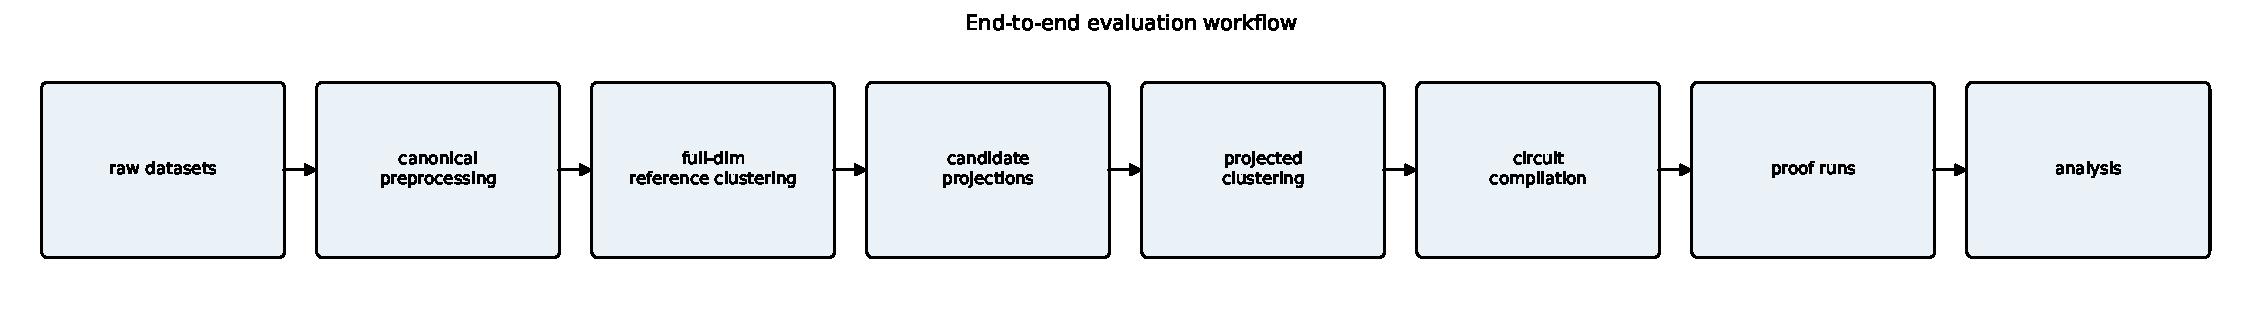
\includegraphics[width=0.91\textwidth]{figures/workflow.pdf}
\caption{End-to-end evaluation workflow.}
\label{fig:End-to-end evaluation workflow}
\end{figure*}}

\clearpage
\subsection{Results}\label{sec:results}

\paragraph{Measured scope.}
The primary evaluation contains eight fixed corpora with the analyzed sizes in Table~\ref{tab:datasets-a}. Proof costs are restricted to completed engineering shapes and explicitly identified row subsets; no full-size MNIST, Fashion-MNIST, Gisette, Arcene, or text-corpus proof is claimed. The follow-up proves 32 Gaussian-easy points, 16 Gaussian-hard points, and eight images from each image corpus, retaining all features. Small-subset fidelity is qualified anew and is not evidence of full-corpus proof fidelity. Missing Pisot reproduction, in-circuit generator, cross-hardware replication, and per-gadget measured constraint/time breakdown are limitations rather than zero-cost entries. Total compiler constraints and compile/setup/prove/verify timings are reported; verifier RSS is scoped to an isolated verifier process where measured.


\subsubsection{RQ1: geometric and clustering fidelity}
\tpexplain{Paragraph 1 --- answer RQ1 in the first sentence with the minimum $m$ meeting a predeclared fidelity threshold. Then explain variations across datasets.}
At the predeclared thresholds $r_\Phi\leq\tau_\Phi$ and $\mathrm{ARI}\geq\tau_{\rm ARI}$, where \decisionplaceholder{fix $\tau_\Phi$ and $\tau_{\rm ARI}$ before inspecting proof-performance results}, \resultplaceholder{method} requires $m=\resultplaceholder{value}$ on \resultplaceholder{dataset/median}, compared with \resultplaceholder{values for baselines}. Fidelity improves \resultplaceholder{monotonically/non-monotonically} with \resultplaceholder{dimension/sparsity}; the principal exception is \resultplaceholder{dataset and reason supported by evidence}.

\begin{table*}[!htbp]
\caption{Clustering fidelity at selected operating points. Report the preregistered point estimate and 95\% confidence interval across seeds.}\label{tab:fidelity-a}
\centering\scriptsize
\begin{adjustbox}{max width=\textwidth}
\begin{tabularx}{\textwidth}{@{}Y Y R R R R R@{}}
\toprule
Dataset & Projection $(m,q)$ & $r_\Phi$ & ARI vs. full & $Q_{0.95}(|\delta|)$ & $\Pr(|\delta|>\epsilon)$ & certified coverage \\
\midrule
\placeholder{dataset} & full & 1.000 & 1.000 & 0 & 0 & 100\% \\
\placeholder{dataset} & PCA $(\_,\_)$ & \resultplaceholder{} & \resultplaceholder{} & \resultplaceholder{} & \resultplaceholder{} & n/a \\
\placeholder{dataset} & dense JL $(\_,\_)$ & \resultplaceholder{} & \resultplaceholder{} & \resultplaceholder{} & \resultplaceholder{} & \resultplaceholder{} \\
\placeholder{dataset} & sparse JL $(\_,\_)$ & \resultplaceholder{} & \resultplaceholder{} & \resultplaceholder{} & \resultplaceholder{} & \resultplaceholder{} \\
\bottomrule
\end{tabularx}
\end{adjustbox}
\end{table*}

\figureplaceholder{Fidelity versus projected dimension}{Small multiples by dataset. Horizontal axis $m$ on log scale; vertical panels for objective ratio, ARI, and 95th-percentile distortion. Lines for each transform with confidence ribbons. Mark the selected deployment point and predeclared acceptability thresholds.}

\subsubsection{RQ2: proof cost and Pareto efficiency}
\tpexplain{Lead with actual wall-clock and memory, then explain constraint counts. Show absolute values as well as speedups.}
On the synthetic $96\times128$ workload at $(m,q)=(16,2)$, sparse JL reduces total constraints by 7.64\%, but median prove-only time is 62.94\,s versus 62.43\,s for full dimension. Setup falls from 728.09\,s to 662.18\,s. No general prove-only speedup is observed; the tiny MNIST subset is 56.33\% slower. These comparisons are scoped to the declared witnesses and repetitions. Measured per-gadget constraint or wall-time attribution is unavailable.

\begin{table*}[!htbp]
\caption{End-to-end proof performance at the fidelity-matched operating point.}\label{tab:zkperf-a}
\centering\scriptsize
\begin{adjustbox}{max width=\textwidth}
\begin{tabularx}{\textwidth}{@{}Y R R R R R R R Y@{}}
\toprule
Method & constraints & witness/compile (s) & proving (s) & peak RAM (GiB) & verify (ms) & proof (KiB) & ARI & Notes \\
\midrule
Full dimension & \resultplaceholder{} & \resultplaceholder{} & \resultplaceholder{} & \resultplaceholder{} & \resultplaceholder{} & \resultplaceholder{} & 1.000 & baseline \\
PCA, public matrix & \resultplaceholder{} & \resultplaceholder{} & \resultplaceholder{} & \resultplaceholder{} & \resultplaceholder{} & \resultplaceholder{} & \resultplaceholder{} & excludes PCA training proof \\
Dense Rade\-macher & \resultplaceholder{} & \resultplaceholder{} & \resultplaceholder{} & \resultplaceholder{} & \resultplaceholder{} & \resultplaceholder{} & \resultplaceholder{} & signed dense \\
Sparse JL & \resultplaceholder{} & \resultplaceholder{} & \resultplaceholder{} & \resultplaceholder{} & \resultplaceholder{} & \resultplaceholder{} & \resultplaceholder{} & proposed \\
Coordinate sample & \resultplaceholder{} & \resultplaceholder{} & \resultplaceholder{} & \resultplaceholder{} & \resultplaceholder{} & \resultplaceholder{} & \resultplaceholder{} & naive lower-cost baseline \\
\bottomrule
\end{tabularx}
\end{adjustbox}
\end{table*}

\figureplaceholder{Proof-cost versus clustering-fidelity Pareto frontier}{Scatter/line plot with proving time or peak RAM on the horizontal axis and original-space objective ratio/ARI on the vertical axis. One symbol per transform and $m$; visually identify nondominated points. Include absolute units and confidence intervals.}

\figureplaceholder{Measured prover stage costs}{Show compile, setup and prove-only timings for completed matched configurations. Report total constraints separately; do not infer per-gadget wall-time or constraint shares from symbolic counts.}

\subsubsection{RQ3: security-ordering overhead}
\tpexplain{Measure the marginal cost of binding data and deriving randomness; do not compare a secure protocol only against itself.}
Post-commitment seed generation adds \resultplaceholder{milliseconds/percentage} to end-to-end latency and \resultplaceholder{constraints/none} to the circuit under the \resultplaceholder{instantiation}. Commitment grinding is evaluated analytically and with \placeholder{bounded-retry simulation}; the selected entropy source prevents the prover from predicting $R$ at binding time under \placeholder{assumption}.

\begin{table*}[!htbp]
\caption{Marginal cost of commit-then-sample ordering. Report zero rather than ``n/a'' when a stage is measured and has no circuit cost.}\label{tab:ordering-a}
\centering\scriptsize
\begin{adjustbox}{max width=\textwidth}
\begin{tabularx}{\textwidth}{@{}Y R R R R Y@{}}
\toprule
Component & host latency (ms) & circuit constraints & transcript bytes & invocations/attempt & Included in end-to-end total \\
\midrule
data/parameter commitment & \resultplaceholder{} & \resultplaceholder{} & \resultplaceholder{} & 1 & yes \\
challenge acquisition & \resultplaceholder{} & 0 & \resultplaceholder{} & 1 & yes \\
sparse-matrix expansion & \resultplaceholder{} & 0 & 0 & 1 & yes \\
matrix authentication & \resultplaceholder{} & \resultplaceholder{} & \resultplaceholder{} & 1 & yes \\
eligibility log/check & \resultplaceholder{} & 0 & \resultplaceholder{} & 1 & yes \\
rejected/retried commitments & \resultplaceholder{} & 0 & \resultplaceholder{} & \resultplaceholder{} & reported separately \\
\bottomrule
\end{tabularx}
\end{adjustbox}
\end{table*}

\subsubsection{RQ4: predictive value of margin conditions}
\begin{table*}[!htbp]
\caption{Validation of assignment and DBSCAN stability certificates. A “violation” means a theorem-certified item changed, which should be zero absent implementation error or a failed embedding event.}\label{tab:cert-a}
\centering\small
\begin{adjustbox}{max width=\textwidth}
\begin{tabularx}{\textwidth}{@{}Y R R R R Y@{}}
\toprule
Dataset/configuration & certified points/pairs & observed stable & uncertified stable & violations & Interpretation \\
\midrule
\placeholder{nearest-centroid case} & \resultplaceholder{} & \resultplaceholder{} & \resultplaceholder{} & \resultplaceholder{} & \placeholder{} \\
\placeholder{low-margin case} & \resultplaceholder{} & \resultplaceholder{} & \resultplaceholder{} & \resultplaceholder{} & \placeholder{} \\
\placeholder{DBSCAN synthetic} & \resultplaceholder{} & \resultplaceholder{} & \resultplaceholder{} & \resultplaceholder{} & \placeholder{} \\
\placeholder{DBSCAN real} & \resultplaceholder{} & \resultplaceholder{} & \resultplaceholder{} & \resultplaceholder{} & \placeholder{} \\
\bottomrule
\end{tabularx}
\end{adjustbox}
\end{table*}

\widefigureplaceholder{Margin, dimension, and exact-preservation phase diagram}{Heatmaps with projection dimension on one axis and synthetic separation/margin on the other. Cells show probability of exact assignment or exact DBSCAN graph preservation across seeds. Overlay the theoretical sufficient-condition boundary.}

\subsubsection{RQ5: sensitivity, scaling, and ablation}
\begin{table*}[!htbp]
\caption{Scaling, sensitivity, and failure quantities required for RQ5.}\label{tab:sensitivity-a}
\centering\scriptsize
\begin{adjustbox}{max width=\textwidth}
\begin{tabularx}{\textwidth}{@{}Y Y Y Y Y@{}}
\toprule
Factor & Declared range & Primary responses & Required numerical summary & Failure/crossover report \\
\midrule
$n,d,k$ & Table~\ref{tab:matrix-a} & prove time, RAM, constraints & descriptive proof slopes; conditional native intervals; absolute endpoints & first timeout/OOM or largest completed size \\
$m,q$ & Table~\ref{tab:matrix-a} & fidelity and proof cost & paired effect and Pareto status & smallest fidelity-eligible $m$ \\
precision & 8--24 bits & $r_\Phi$, mismatch, constraints & error/cost change from reference precision & first failed range or fidelity target \\
cluster separation & declared $\gamma$ grid & ARI, agreement, certificate coverage & effect by margin bin & margin at target stability \\
backend/hardware & one server; primary Groth16 and separately scoped tiny backend pilot & absolute time/RAM & descriptive matched ratios; no cross-hardware inference & no large backend comparison \\
\bottomrule
\end{tabularx}
\end{adjustbox}
\end{table*}

\begin{table*}[!htbp]
\caption{Ablation study at one representative and one stress-test configuration.}\label{tab:ablation-a}
\centering\small
\begin{adjustbox}{max width=\textwidth}
\begin{tabularx}{\textwidth}{@{}Y R R R R Y@{}}
\toprule
Variant removed/changed & proving (s) & RAM (GiB) & constraints & fidelity & Conclusion \\
\midrule
Full CommitJL & \resultplaceholder{} & \resultplaceholder{} & \resultplaceholder{} & \resultplaceholder{} & reference \\
Dense instead of sparse & \resultplaceholder{} & \resultplaceholder{} & \resultplaceholder{} & \resultplaceholder{} & isolates sparsity \\
Pre-published instead of post-commit $R$ & \resultplaceholder{} & \resultplaceholder{} & \resultplaceholder{} & same & isolates security overhead \\
No range-check batching & \resultplaceholder{} & \resultplaceholder{} & \resultplaceholder{} & same & implementation optimization \\
Lower precision & \resultplaceholder{} & \resultplaceholder{} & \resultplaceholder{} & \resultplaceholder{} & quantization trade-off \\
\bottomrule
\end{tabularx}
\end{adjustbox}
\end{table*}

\widefigureplaceholder{Scaling and sensitivity dashboard}{Four panels: proving time vs. $n$; proving time vs. $d$; fidelity vs. $q$; fidelity/proving cost vs. precision. Show asymptotic guide lines and mark timeout/OOM points explicitly.}

\subsection{Discussion}\label{sec:discussion}

\subsubsection{What the evidence would and would not establish}
\tpexplain{Interpret the central trade-off conservatively. State the deployment regime where the method wins and where full dimension/PCA is preferable.}
CommitJL can help only if the saved downstream proof work exceeds the cost of commitment, matrix generation, and projection, and if the resulting geometric error is acceptable. This is most plausible for large $d$, moderate $m$, repeated distance calculations, and well-separated clusters. Full-dimensional computation or PCA may be preferable for low-dimensional data, small margins, or backends with cheap dense linear operations.

\subsubsection{Security and privacy limitations}
\tpexplain{Discuss leakage from output, seed bias/grinding, denial of service, malicious verifier parameters, and trusted setup if applicable.}
The protocol does not make the public cost private; output leakage may require a separately analyzed privacy mechanism or access control. Commit-then-sample prevents adaptation after an eligible commitment but does not eliminate grinding unless the deployment enforces the stated budget $Q$ and eligibility policy. It also does not prevent denial-of-service inputs or malicious application choices that are already contained in the recorded public parameters. Security inherits the assumptions and setup model of \placeholder{selected proof system}. The draft therefore makes no differential-privacy, fairness, or unbounded selective-abort-resistance claim.

\subsubsection{Validity threats}
\begin{table}[!htbp]
\caption{Threats to validity and mitigation measures.}\label{tab:validity-a}
\centering\scriptsize
\begin{tabularx}{\columnwidth}{@{}Y Y@{}}
\toprule
Threat & Mitigation \\
\midrule
ARI/objective omit application loss & report geometry, clustering, certificates, and downstream metrics \\
Native/circuit arithmetic differs & golden vectors, differential tests, checked ranges \\
Warm-up or caching biases time & isolated runs, fixed warm-up, raw logs \\
Few backends or platforms & one complete backend; symbolic model; optional second backend \\
Benchmarks underrepresent production & synthetic scaling; explicit extrapolation limits \\
Seeds or initializations are selected & preregister grid; paired seeds; publish failures and all runs \\
JL theorem mismatches generator & distribution audit; theorem-specific tests; conditional claims \\
\bottomrule
\end{tabularx}
\end{table}

\subsubsection{Reproducibility and artifact plan}
\tpexplain{List the exact artifacts required to reproduce every table and figure.}
The artifact will contain circuit source, native reference code, dataset manifests, generator test vectors, environment lockfiles, hardware metadata, raw run logs, analysis scripts, and one command per paper table/figure. Random seeds and failed runs will be archived. \newtext{Concretely, the code repository is laid out as \texttt{commitjl/} (core Python package: encoding, hashing, commit, sparse\_gen, randomness, quantize, protocol, projections, clustering, certificates, metrics, stats, cost\_model, zk\_bridge), \texttt{zk/} (Go/gnark circuit in \texttt{zk/circuit} and CLI \texttt{zk/cmd/commitjl-prove}), \texttt{data/loaders.py} (dataset loaders and SHA256 manifest), \texttt{experiments/} (config-driven grid runners \texttt{rq1\_fidelity.py}--\texttt{rq5\_scaling.py} and \texttt{ablation.py}, plus \texttt{make\_tables.py} and \texttt{make\_figures.py}), \texttt{figures/schematics.py} (conceptual diagrams), and \texttt{results/\{tables,figures\}} (generated outputs) with \texttt{results/*.parquet} raw per-row data and \texttt{results/headline.json} an abstract-ready summary annotated by \texttt{env\_capture.py}. Grids are driven by three config files, \texttt{experiments/configs/\{smoke,native,core\}.yaml}, plus the preregistered analysis parameters in \texttt{experiments/configs/prereg.yaml} ($\epsilon=0.15$, $\tau_\Phi=0.10$, $\tau_{\rm ARI}=0.80$, pair-set size 2000, core-grid selection rule ``smallest $m$ meeting $\tau_{\rm ARI}$ and $\tau_\Phi$'', seed 12345, 10 native repetitions, 10 proof repetitions with 1 warm-up). Each table/figure is reproduced with \texttt{make native}, \texttt{make core}, and then \texttt{make tables figures}, or individually via \texttt{python -m experiments.make\_tables --table <label>} (labels: fidelity-a, zkperf-a, ordering-a, cert-a, sensitivity-a, ablation-a, datasets-a, circuit-cost, validity-a) and \texttt{python -m experiments.make\_figures --fig <label>} (labels: fidelity-vs-m, pareto, cost-breakdown, phase-diagram, plus the scaling/sensitivity dashboard); \texttt{python -m figures.schematics --diagram <label>} independently regenerates the seven hand-drawn conceptual figures (protocol, security\_game, generator, dataflow, architecture, workflow, motivation). Every dataset loaded by \texttt{data/loaders.py} is recorded in a SHA256 manifest entry (array hash plus name/$n$/$d$/$k$/source) so each reported row is traceable to a fixed data hash; the manifest is regenerated automatically on first load into \texttt{COMMITJL\_DATA} and is not a fixed value we can quote until the datasets in Table~\ref{tab:datasets-a} are finalized.} \placeholder{Repository DOI and anonymous-review URL.}

\figureplaceholder{Decision guide for practitioners}{A compact decision tree: Is $d$ large? Is approximate clustering acceptable? Is there post-commit public entropy? Are margins sufficient? Is the projection reused? Leaves recommend full dimension, PCA, CommitJL, or further validation. Base thresholds on measured crossover points.}

\section{Conclusion}\label{sec:conclusion}
\tpexplain{One paragraph: problem, method, strongest result, theoretical boundary, and one future direction. Do not introduce new baselines or claims.}
CommitJL aligns the protocol order with the assumption behind random projection: both the data and fixed centers are bound before the transform is sampled. It authenticates the verifier-derived sparse matrix, proves the projected computation, and treats fidelity to the original space as a separate geometric claim. Across \placeholder{datasets/backends}, the method achieves \resultplaceholder{main cost result} at \resultplaceholder{main fidelity result}; \placeholder{measured crossover/margin condition} marks the observed boundary of its useful regime. The present construction covers fixed-centroid auditing. Extending it to \placeholder{private model learning, scalable DBSCAN, alternative proof backends, or differential privacy} remains future work.

\backmatter

\begin{appendices}
\section{Formal security game and proof}\label{app:security-a}
\paragraph{Game.} The challenger runs setup and publishes parameters. For a task identifier, the adversary may register at most $Q$ eligible pairs $(C_X,C_\theta)$ before the corresponding challenge is known. For each eligible pair, the challenger samples an independent $\rho\leftarrow\{0,1\}^{256}$, derives $A$ and $C_A$, and returns the public transcript. An abort consumes that attempt. The adversary wins if any submitted $(\widehat\Psi,\pi)$ verifies although no tuple $(X,r_X,A,a_1,\ldots,a_n)$ opens $C_X$, authenticates to the verifier-derived $C_A$, and satisfies the exact relation in Section~\ref{sec:background}.

\begin{proof}[Proof of Theorem~\ref{thm:composition-a}: cryptographic part]
Fix one eligible transcript, and let $F$ be the event that the verifier accepts a value $\widehat\Psi$ not equal to the relation's output on the dataset fixed by $C_X$ and the matrix derived by the verifier. Knowledge soundness supplies, except with probability $\delta_{\rm ks}$, an extracted witness satisfying every circuit constraint for the accepted public statement. Call this event $K$.

Condition on $K$. If the extracted opening and the value fixed by $C_X$ are different canonical encodings, the two valid openings break commitment binding; this event has probability at most $\delta_{\rm bind}$. Otherwise the extracted $X$ is the committed dataset. If the public parameters used by the relation differ from the parameters registered before the challenge but have the same $C_\theta$, they give a collision in $H_\theta$. The verifier deterministically computes $A$ and $C_A$ from the recorded transcript. If the extracted sparse list differs from $A$ but hashes to $C_A$, it gives a collision in $H_A$. Let $\delta_{\rm hash}$ bound the union of these two collision events. Outside these bad events, the satisfied relation uses the registered parameters and verifier-derived matrix, enforces every lowest-index argmin, and checks
$\widehat\Psi=\sum_i\|A(x_i-c_{a_i})\|_2^2$.
Hence $F\subseteq\neg K\cup F_{\rm bind}\cup F_{\rm hash}$, and the union bound gives
\[
\Pr[F]\le\delta_{\rm ks}+\delta_{\rm bind}+\delta_{\rm hash}.
\]
The post-commit challenge makes the geometric draw independent of the already fixed data and centers; it is not needed to infer circuit satisfaction. In the ideal-generator experiment, adding $\Pr[\neg\mathcal E_\epsilon]=\delta_{\rm geom}$ bounds the union of cryptographic and geometric failure for one transcript. A concrete XOF replacement adds $\operatorname{Adv}_{\rm xof}$ by a real/ideal hybrid. Applying the union bound to at most $Q$ eligible transcripts yields the task-level bound in the theorem. No independence-based product bound is claimed.
\end{proof}

\section{Detailed geometric and arithmetic proofs}\label{app:geometry-a}
\begin{proof}[Proof of Proposition~\ref{prop:unbiased-a}]
Write $h_\ell(t)$ and $\sigma_\ell(t)$ for the row and sign of the $\ell$th nonzero in column $t$. Expanding by output row gives
\begin{align*}
\|Av\|_2^2
={}&\sum_{r=1}^{m}\sum_{t,u=1}^{d}\sum_{\ell,a=1}^{q}
\mathbf 1[h_\ell(t)=r]\mathbf 1[h_a(u)=r]\\
&\qquad{}\cdot\sigma_\ell(t)\sigma_a(u)v_tv_u.
\end{align*}
Condition on all row choices. When $(t,\ell)\ne(u,a)$, independence and zero mean of the signs give
$\mathbb E[\sigma_\ell(t)\sigma_a(u)]=0$. When $(t,\ell)=(u,a)$, the product is one and exactly one row indicator is active. Hence
\[
\mathbb E[\|Av\|_2^2\mid h]
=\sum_{t=1}^{d}\sum_{\ell=1}^{q}v_t^2
=q\|v\|_2^2.
\]
Taking expectation over the row choices and dividing by $q$ proves the claim. The argument establishes only the first moment and therefore does not replace a concentration analysis.
\end{proof}

\begin{lemma}[Fixed-center nearest-cost preservation]\label{lem:fixed-cost-a}
If $\mathcal E_\epsilon(A;D(X,\mathcal C))$ holds, then
$(1-\epsilon)\Phi_X(\mathcal C)\le q^{-1}\Phi_{AX}(A\mathcal C)\le(1+\epsilon)\Phi_X(\mathcal C)$.
\end{lemma}
\begin{proof}
For each $i,j$, define $d_{ij}=\|x_i-c_j\|_2^2$ and $d'_{ij}=q^{-1}\|A(x_i-c_j)\|_2^2$. The event gives $(1-\epsilon)d_{ij}\le d'_{ij}\le(1+\epsilon)d_{ij}$. Let $j_i\in\arg\min_jd_{ij}$ and $j'_i\in\arg\min_jd'_{ij}$. For the upper bound,
$\min_jd'_{ij}=d'_{ij'_i}\le d'_{ij_i}\le(1+\epsilon)d_{ij_i}=(1+\epsilon)\min_jd_{ij}$.
For the lower bound, every $j$ satisfies $d'_{ij}\ge(1-\epsilon)d_{ij}\ge(1-\epsilon)\min_\ell d_{i\ell}$; taking the minimum over $j$ preserves this inequality. Summing both pointwise bounds over $i$ proves the claim. Combining it with the cryptographic part above proves the geometric conclusion of Theorem~\ref{thm:composition-a}.
\end{proof}

\begin{lemma}[Nearest-centroid margin]\label{lem:margin-a}
Let $c_1$ be the unique nearest center to $x$, with distance $d_1$, and let $d_2$ be the distance to the closest competing center. Under $\mathcal E_\epsilon$, the projected lowest-index argmin remains $c_1$ whenever $d_1=0<d_2$, or $d_1>0$ and $d_2^2/d_1^2>(1+\epsilon)/(1-\epsilon)$.
\end{lemma}
\begin{proof}
If $d_1=0$, linearity gives $A(x-c_1)=0$, while $d_2>0$ and $\epsilon<1$ imply every competitor has projected squared distance at least $q(1-\epsilon)d_2^2>0$. If $d_1>0$, the stated ratio is equivalent to $(1+\epsilon)d_1^2<(1-\epsilon)d_2^2$. The projected squared distance to $c_1$, divided by $q$, is at most the left side; that to every competitor is at least the right side. The projected comparison is therefore strict. Original ties are intentionally excluded: a deterministic tie rule makes execution well-defined but distortion alone cannot certify that a tie remains a tie.
\end{proof}

\begin{lemma}[DBSCAN graph preservation]\label{lem:dbscan-a}
Assume $\mathcal E_\epsilon$ holds for all pair differences and no squared pair distance lies in $[\rho^2/(1+\epsilon),\rho^2/(1-\epsilon)]$. Then the original and projected radius-$\rho$ neighborhood graphs are identical. With the same $\mathrm{minPts}$, vertex order, queue order, and border-point tie rule, deterministic DBSCAN returns identical labels.
\end{lemma}
\begin{proof}
For a neighbor, the no-band assumption strengthens $\|x_i-x_j\|^2\le\rho^2$ to $\|x_i-x_j\|^2<\rho^2/(1+\epsilon)$; hence $q^{-1}\|A(x_i-x_j)\|^2<\rho^2$. For a non-neighbor, the adopted edge rule is $\|x_i-x_j\|\le\rho$, so non-neighbor means squared distance $>\rho^2$; no-band strengthens it to $>\rho^2/(1-\epsilon)$, hence the projected value is $>\rho^2$. Every adjacency bit is equal. Therefore neighbor counts and core predicates are equal. A deterministic traversal given the same graph, order, and border-point rule executes the same state transitions and produces the same labels \cite{ester1996dbscan}.
\end{proof}

\begin{lemma}[Quantization perturbation]\label{lem:quant-a}
If each coordinate is rounded with absolute error at most $1/(2S)$, then for any real $u,v$ and their decoded quantizations $\tilde u/S,\tilde v/S$,
\begin{align*}
&\left|\|\tilde u/S-\tilde v/S\|_2^2-\|u-v\|_2^2\right|\\
&\hspace{2em}\le 2\|u-v\|_2\sqrt d/S+d/S^2.
\end{align*}
\end{lemma}
\begin{proof}
Write $\tilde u/S=u+e_u$, $\tilde v/S=v+e_v$, and $e=e_u-e_v$. Coordinatewise, $|e_t|\le1/S$, so $\|e\|_2\le\sqrt d/S$. With $w=u-v$,
$\|w+e\|_2^2-\|w\|_2^2=2\langle w,e\rangle+\|e\|_2^2$.
Taking absolute values, applying Cauchy--Schwarz, and substituting the bound on $\|e\|_2$ gives the result. This error is additive and must be composed separately with multiplicative projection distortion.
\end{proof}

\paragraph{No-wraparound certificate.} If $|x_t|,|c_t|\le B$, the no-duplicate-row rule permits at most one contribution from each input coordinate to a fixed output row. A row accumulator for $A(x_i-c_j)$ therefore contains at most $d$ signed contributions of magnitude at most $2B$, so its magnitude is at most $2dB$. Its squared norm is at most $D_{\max}=4md^2B^2$; a difference of two candidate distances has magnitude at most $2D_{\max}$; and the reported sum is at most $\Psi_{\max}=nD_{\max}$. Canonical signed decoding agrees with integer arithmetic when these quantities are range-checked and $p>2\max\{2dB,2D_{\max},\Psi_{\max}\}$. The final artifact must instantiate $B,S,p$ and the gadget bit widths; until then this is a symbolic obligation, not an implementation claim.

\section{Complete experimental configurations}
\tpexplain{Provide every hyperparameter, dataset checksum, preprocessing choice, command, hardware/software version, and excluded/failed run.}
The completed primary native grid uses 10 projection seeds, 5 paired clustering initializations, $q\in\{1,2,4\}$, and every valid $m\in\{16,32,64,128,256,512,1024\}$ at or below $d$. The targeted follow-up adds $q=8$ on three corpora and $m=1536$ where valid. The native operating-point selection uses the smallest $m$ meeting confidence-bound fidelity thresholds without proof timings. The completed proof grids are explicitly resource-bounded engineering shapes and separately qualified row subsets; adjacent-dimension coverage is not claimed. Each proof configuration receives one warm-up and the campaign-specific 3, 5, or 10 measured runs. \newtext{These per-condition repetition counts (\texttt{n\_reps\_native: 10}, \texttt{n\_reps\_proof: 10}, \texttt{n\_warmup\_proof: 1}) and the fidelity thresholds ($\tau_\Phi=0.10$, $\tau_{\rm ARI}=0.80$, JL-distortion tolerance $\epsilon=0.15$, preregistered pair-set size 2000, master seed 12345) are fixed in \texttt{experiments/configs/prereg.yaml} and are read, not re-chosen, by \texttt{experiments/rq2\_proof\_cost.py}'s core-grid selection.} A run manifest records dataset checksum and license, preprocessing parameters, split indices, all seeds, compiler and dependency versions, circuit hash, hardware and OS identifiers, start/end timestamps, exit status, timeout/OOM reason, raw counters, proof hash, and verification result. \newtext{Each \texttt{experiments/rq*.py} script is resumable (it skips rows already present in its output parquet, keyed by a config hash) and shardable, e.g.\ \texttt{python -m experiments.rq2\_proof\_cost --config experiments/configs/core.yaml --shard 1/4}; environment/version capture (\texttt{env\_capture.py}) and dataset hashing (\texttt{data/loaders.py}) are wired into every run rather than recorded by hand.} Hardware, backend, repository, and dataset checksums remain placeholders until the implementation and artifacts exist.

Before submission, every RQ must have its primary endpoint, denominator, absolute baseline value, paired effect, uncertainty interval, attempted-run count, and failure count. Every reported operating point must identify $(m,q)$, precision, clustering parameters, backend, hardware, and seed set. The abstract and conclusion must use the same fidelity-matched configuration as the main tables; a faster but fidelity-ineligible configuration may be reported only as a trade-off point, not as the headline result.
\end{appendices}

\bmhead{Acknowledgements}
\placeholder{Acknowledge research assistance, infrastructure access, and non-author contributions. Do not repeat funding information here unless required by the funder.}

\bmhead{Author contributions}
\placeholder{Use full author names and CRediT-style roles: conceptualization, methodology, software, validation, formal analysis, investigation, writing, visualization, and supervision.}

\bmhead{Data availability}
The public datasets analyzed in this study are available from the repositories cited in Table~\ref{tab:datasets-a}. Generated datasets, processed manifests, and raw experimental results will be archived at \placeholder{repository and persistent URL}.

\bmhead{Code availability}
Source code, circuit definitions, scripts, and environment specifications will be archived at \placeholder{repository and DOI}.

\bmhead{Materials availability}
The circuits, configuration manifests, generated instances, and supplementary artifacts will be available at \placeholder{repository and DOI}. \placeholder{State any redistribution restrictions.}

\section*{Declarations}
\bmhead{Funding}
\placeholder{The authors declare that no funds, grants, or other support were received / insert funder and grant number.}

\bmhead{Conflict of interest}
The authors have no relevant financial or non-financial interests to disclose. \placeholder{Confirm for all authors.}

\bmhead{Ethics approval and consent to participate}
Not applicable. \placeholder{Reassess if human-derived sensitive data are added.}

\bmhead{Consent for publication}
Not applicable.

% Author information is generated from the \author and \affil metadata above.
% Additional information is publisher-generated metadata and is not inserted
% as a manuscript section.

\bibliography{references}

\end{document}